\documentclass[table]{beamer}
\usetheme{defense}
\graphicspath{{../../figures/}}

\newcommand{\leftRect}[2]{\node[draw=text,very thick,rounded corners, text width=0.46\textwidth,minimum height=6cm] at (0,0) {\centering\textbf{#1}\\ \raggedright \color{text}#2};}
\newcommand{\rightRect}[2]{\node[draw=text,very thick,rounded corners, text width=0.46\textwidth,minimum height=6cm] at (0.54\textwidth,0) {\centering\textbf{#1}\\ \raggedright \color{text}#2};}

\usepackage{tikz}

\title{Memristors-based recurent modules for neural computing}

\subtitle{}

\institute[IST]{%
  Diogo Caetano\\
  INESC-MN
  \and{}%
  Ruxandra Barlulescu\\
  INESC-ID
  }
  \author[V. BARBAZA]{Valentin BARBAZA}

  \date{17/11/2023}

  \logo{
    \begin{tikzpicture}[overlay,remember picture]
      \node[left=0cm] at (current page.33){
        
\includegraphics[height=1cm]{logos/inesc-mn.png}
        \hspace{1pt}
        
\includegraphics[height=1cm]{logos/ist.eps}
        
\includegraphics[height=1cm]{logos/inesc-id.eps}
      };
    \end{tikzpicture}
  }

  \begin{document}

  \frame{\titlepage}

  \begin{frame}
    \frametitle{Table of Contents}
    \tableofcontents
  \end{frame}

  \section{Motivation and objectives}
  \begin{frame}{\insertsection}{\insertsubsection}
    The goal of the thesis is to know whether an analog LSTM network would work. This would allow running a Neural Network in real-time in embedded systems. The analog implementation (using memristors crossbar array) allows for much greater computational speed and very small on-chip area.
  \end{frame}
  \section{The circuits}
  \subsection{Activation functions}
  \begin{frame}{\insertsection}{\insertsubsection}
    My point is to run simulations using cadence. Running a working simulation is the first step before fabricating the system.
  \end{frame}
  \section{The tools}
  \begin{frame}{\insertsection}{\insertsubsection}
    So far, I have designed some smaller elements required for the system to work such as the activation function for example.\\
    I've designed a full size LSTM (with 4 hidden state).
    \begin{figure}
      \centering
      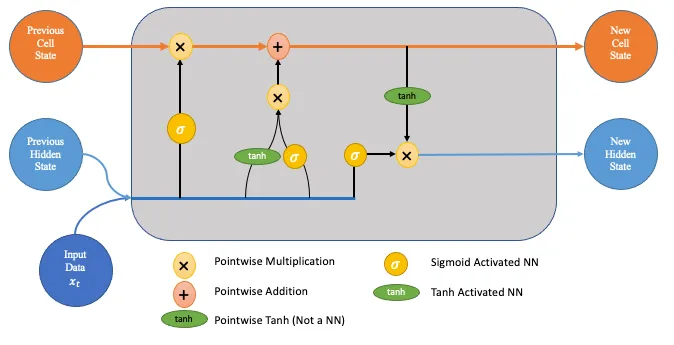
\includegraphics[height=0.35\textheight]{lstm/lstm.png}
    \end{figure}
    I am now working on a way to generate LSTM network of any size.
  \end{frame}

  \section{The datasets}
  \begin{frame}{\insertsection}{\insertsubsection}
    I now need to run the simulations and compare the results of my simulation with the results a digital LSTM (running with Keras for example).
  \end{frame}

  \subsection{Tressk}
  \begin{frame}{jdjd}{}
  \end{frame}

  \end{document}
